% **************************************************
% Macro specifiche per il documento corrente
% **************************************************
% Nome
\newcommand{\docName}{Piano di Qualifica}
% Nome file
\newcommand{\docFileName}{piano\_di\_qualifica.1.1.pdf}
% Versione
\newcommand{\docVers}{1.1}
% Data creazione
\newcommand{\creationDate}{2012-12-10}
% Data ultima modifica
\newcommand{\modificationDate}{2012-12-18}
% Stato in {Approvato, Non approvato}
\newcommand{\docState}{Approvato}
% Uso in {Interno, Esterno}
\newcommand{\docUsage}{Esterno}
% Destinatari da specificare come nome1\\ &nome2\\ ecc.
\newcommand{\docDistributionList}{Proponente\\ &Committente}
% Redattori da specificare come nome1\\ &nome2\\ ecc.
\newcommand{\docAuthors}{Stefano Farronato\\ &Riccardo Tresoldi}
% Approvato da
\newcommand{\approvedBy}{Elena Zecchinato}
% Verificatori
\newcommand{\verifiedBy}{Diego Beraldin}
% Perscorso (relativo o assoluto) che punta alla directory contenente shared/
% come sua sottodirectory (per comodità chiamiamola 'doc root').
\newcommand{\docRoot}{..}
% definire se si vuole l'indice delle tabelle
\def\INDICETABELLE{false}
% definire se si vuole l'indice delle figure
\def\INDICEFIGURE{false}

% importa il preambolo condiviso da tutti i documenti
% shared/preamble.tex
%
% Questo documento contiene la parte del preambolo condivisa e viene pertanto
% richiamato nel 'master' di tutti i documenti di progetto.  Al suo interno
% contiene le inclusioni (e le configurazioni) di tutti i package richiesti per
% la compilazione dei documenti, le macro di carattere generale e la definizione
% degli stili di pagina.

\documentclass[a4paper,10pt,openright]{article}

% **************************************************
% Macro generiche
% **************************************************
\newcommand{\team}{Software Synthesis}                    % chi siamo
\newcommand{\email}{software.synthesis@gmail.com}         % e-mail
\newcommand{\caName}{}                                    % titolo capitolato
\newcommand{\caDescr}{}                                   % descrizione
\newcommand{\inglese}[1]{\textit{#1}}

% **************************************************
% Codifica e lingua dei documenti
% **************************************************
\usepackage[utf8x]{inputenc}                              % codifica caratteri dei documenti sorgenti
\usepackage[english,italian]{babel}                       % localizzazione ai fini di sillabazione e cross-references
\usepackage[T1]{fontenc}                                  % codifica font di output

% **************************************************
% Definizione geometria della pagina
% **************************************************
\usepackage[a4paper,head=4cm,top=4.5cm,bottom=3cm,left=3cm,right=3cm,bindingoffset=5mm]{geometry}

% *************************************************
% Intestazioni e piè di pagina personalizzati
% *************************************************
\usepackage{fancyhdr}
% stile normale
\fancypagestyle{normal}{
\fancyhead{}                                              % intestazione
\fancyhead[RE,RO]{
\begin{picture}(0,0)
  \put(-410,0){
\includegraphics[width=1.02\textwidth]{header_logo}}
  \put(-410,10){\sffamily\large\leftmark}
\end{picture}
\vspace{-4pt}
}
\renewcommand{\headrulewidth}{.4pt}                       % riga sotto l'intestazione
\cfoot{}                                                  % piè di pagina
\fancyfoot[RO,LE]{\sffamily
  pag.~\thepage{} di \pageref{LastPage}}                  % a dx nelle pag. dispari e a sx in quelle pari
\fancyfoot[RE,LO]{\sffamily\docFileName{} -- v.\docVers}
\renewcommand{\footrulewidth}{.4pt}                       % riga sopra il piè di pagina
}
% stile per gli indici
\fancypagestyle{toc}{
\fancyhead{}                                              % intestazione
\fancyhead[RE,RO]{
\begin{picture}(0,0)
  \put(-410,0){
\includegraphics[width=1.02\textwidth]{header_logo}}
\end{picture}
}
\renewcommand{\headrule}{}                                % nessuna riga sotto l'intestazione
\cfoot{}                                                  % piè di pagina
\fancyfoot[RO,LE]{\sffamily\thepage{}}                    % a dx nelle pag. dispari e a sx in quelle pari
\fancyfoot[RE,LO]{\sffamily\docFileName{} -- v.\docVers}
\renewcommand{\footrulewidth}{.4pt}                       % riga sopra il piè di pagina
}

\pagestyle{fancy}                                         % premetto: non so usare bene le marche:
\renewcommand{\sectionmark}[1]{\markboth{#1}{#1}}         % se qualcuno ha idee migliori si faccia avanti!

% **************************************************
% Tabelle
% **************************************************
\usepackage{tabularx}                                     % tabelle di larghezza fissa con una o più colonne variabili
\usepackage{multirow}                                     % colonne con colonne che si estendono per più righe
\usepackage{booktabs}                                     % per inserire l'ambiente table e le righe orizz. nelle tabelle
\usepackage{longtable}			                          % tabelle oltre i limiti di pagina

% **************************************************
% Cross-references e collegamenti ipertestuali
% **************************************************
\usepackage[hidelinks]{hyperref}
\hypersetup{%
  colorlinks=false, linktocpage=false, pdfborder={0,0,0}, pdfstartpage=3, pdfstartview=FitV,%
  urlcolor=Cyan, linkcolor=Cyan, citecolor=Black, %pagecolor=Black,%
  pdftitle={\docName}, pdfauthor={\team}, pdfsubject={}, pdfkeywords={},%
  pdfcreator={pdflatex}, pdfproducer={pdflatex with hyperref package}%
}

% **************************************************
% Immagini e grafica
% **************************************************
\usepackage{graphicx}                                     % supporto ad aspetti avanzati delle immagini
\graphicspath{{\docRoot/pics/}}                           % percorso contenente tutti i file immagini
\usepackage{color}                                        % permette di colorare facilmente il testo

% **************************************************
% Altri pacchetti opzionali
% **************************************************     
\usepackage{lastpage}                                     % per sapere il numero totale di pagine
\usepackage{lipsum}                                       % genera "dummy text" per prove di impaginazione
\usepackage{eurosym}                                      % per il simbolo dell'euro usare \EUR{x} dove x è l'importo


% Fine del preambolo e inizio del documento
\begin{document}

% Inclusione della prima pagina
% shared/firstpage.tex
%
% Questo documento definisce il contenuto della prima pagina, che si suppone
% essere uguale in tutti i documenti.  Oltre al logo e al titolo, la prima
% pagina contiene i metadati relativi al documento in cui viene inclusa.


% rimuove intestazioni e piè di pagina
\pagestyle{empty}

\begin{center}

% logo del gruppo

\includegraphics[width=1.5\textwidth]{logo}

\vspace{1in}

% titolo del documento
{\Huge\bfseries \docName}

\vspace{1in}

% tabella riepilogativa
\begin{tabularx}{.7\textwidth}{>{\bfseries\sffamily}l>{\sffamily}l}
\toprule
\multicolumn{2}{>{\sffamily}c}{Informazioni sul documento}\\
\midrule
Nome file:            & \docFileName\\
Versione:             & \docVers\\
Data creazione:       & \creationDate\\
Data ultima modifica: & \modificationDate\\
Stato:                & \docState\\
Uso:                  & \docUsage\\
Redattori:            & \docAuthors\\
Approvato da:         & \approvedBy\\
Verificatori:         & \verifiedBy\\
\bottomrule
\end{tabularx}

\end{center}

\newpage


% Storico delle modifiche
\section*{Storia delle modifiche}
\begin{longtable}{lp{.3\textwidth}lll}
\toprule
Versione & Descrizione intervento & Redattore & Ruolo & Data\\
\midrule % inserire qui il contenuto della tabella
% TODO: questa riga deve essere completata
1.1 & Stesura sezione qualità di processo & & & 2012-12-15\\
1.0 & Approvazione documento & Elena Zecchinato & & 2012-12-18\\
0.12 & Correzione errori segnalati dal verificatore & Stefano Farronato & & 2012-12-18\\
0.11 & Verifica Capitoli 5,6,7,8,9 & Diego Beraldin & & 2012-12-17\\
0.10 & Verifica Capitoli 1,2,3,4 & Diego Beraldin & & 2012-12-16\\
0.9 & Correzione paragrafo 4.1 e paragrafo 6.1 & Riccardo Tresoldi & & 2012-12-15\\
0.8 & Correzione paragrafo 6.3 e stesura capitolo ''Riferimenti''& Stefano Farronato & & 2012-12-14\\
0.7 & Impostazione capitoli rimanenti: ``Resoconto delle attività di verifica'', ``Prossima versione Piano di Qualifica''. Correzione paragrafo 6.2.1. & Riccardo Tresoldi & & 2012-12-13\\
0.6 & Correzione capitolo ``Visione generale della strategia di verifica'' nella ``risorse necessarie e disponibili'' & Riccardo Tresoldi & & 2012-12-12\\
0.5 & Stesura capitolo ``Gestione amministrativa della revisione''& Stefano Farronato & & 2012-12-12\\
0.4 & Stesura capitolo ``Strumenti, tecniche e metodi '', conclusione capitolo ``Obiettivi di qualità'' & Riccardo Tresoldi & & 2012-12-11\\
0.3 & Stesura capitolo ``Qualità'' & Stefano Farronato & & 2012-12-11\\
0.2 & Stesura capitolo ``Visione generale della strategia di verifica'' & Stefano Farronato & & 2012-12-10\\
0.1 & Stesura scheletro documento, introduzione & Stefano Farronato & & 2012-12-10\\
\bottomrule
\end{longtable}
\newpage

% inclusione dell'indice
% shared/toc.tex
%
% Questo file contiene le istruzioni che generano l'indice o gli indici del
% documento (utile nel caso in cui decidessimo di avere anche un indice delle
% tabelle e/o un indice delle figure).

\pagestyle{toc}
\pagenumbering{roman}

\tableofcontents

\newpage


% Alcuni aggiustamenti per le pagine
\pagenumbering{arabic}
\setcounter{page}{1}
\pagestyle{normal}

% Qui ha inizio il documento vero e proprio...
\section{Introduzione}
\subsection{Scopo del prodotto}
\purpose

\subsection{Scopo del documento}

Il seguente documento ha lo scopo di presentare la strategia di verifica e di validazione complessiva che utilizzeranno i componenti del team di lavoro di Software Synthesis a scopo di garantire la qualità richiesta nello svolgimento del progetto MyTalk regolarmente accettato dall'azienda appaltatrice Zucchetti s.r.l.

Durante lo svolgimento del suddetto progetto sarà possibile l'insorgere di modifiche a tale documento, dettate da eventuali scelte progettuali o da esplicite richieste del committente stesso.

\subsection{Glossario}
\glossaryIntro
\clearpage

\section{Riferimenti}

\subsection{Normativi}

\begin{itemize}
\item[] \textit{norme\_di\_progetto.1.0.pdf} allegato;
\item[]  Verbale \textit{verbale\_incontro\_2012-12-11.pdf} allegato;
\item[]  Riferimenti a specifici estratti del testo \textit{Software Engineering (8th edition) Ian Sommerville, Pearson Education | Addison-Wesley} quali:
\begin{itemize}
\item[]  \textit{ISO/IEC 9126:2001, Software engineering - Product quality - Part 1: Quality model};
\item[]  \textit{ISO/IEC 12207, Software Life Cycle Processes}.
\end{itemize}
\end{itemize}

\subsection{Informativi}

\begin{itemize}
\item[] \textit{analisi\_dei\_requisiti.1.0.pdf};
\item[] \textit{piano\_di\_progetto.1.0.pdf};
\item[] \textit{glosssario1.0.pdf};
\item[] Capitolato d'appalto: MyTalk, v 1.0, redatto e rilasciato dal proponente Zucchetti S.r.l reperibile all'indirizzo: \url{http://www.math.unipd.it/~tullio/IS-1/2012/Progetto/C1.pdf};

Riferimenti a specifici estratti del testo \textit{Software Engineering (8th edition) Ian Sommerville, Pearson Education | Addison-Wesley} quali:

\begin{itemize}
\item[]  \textit{Software Engineering - Part 5: Verification and Validation, Part 6: Management}.\\
\end{itemize}
\end{itemize}
\clearpage

\section{Obiettivi di qualità}
% TODO: Controllare che tutti questi requisiti aggiuntivi siano presenti anche nell'analisi dei requisiti

\subsection{Qualità di processo}
% scrivere parte sulla qualità di processo con SPA-I e CMMI

\subsection{Qualità di prodotto software}
Al fine di garantire un elevato standard qualitativo, sia per ovvia scelta del team di sviluppo, sia per implicita richiesta da parte del committente stesso, Software Synthesis ha preso come riferimento lo standard ISO/9126:2001.

\begin{description}
\item{\bfseries Funzionalità}
Il prodotto MyTalk deve soddisfare nelle sue funzionalità tutti i requisiti individuati nell'attività di Analisi, garantendone il funzionamento e l'aderenza alle richieste specifiche del committente. Tutto questo sarà svolto nel modo meno oneroso sia dal punto di vista economico che di sfruttamento delle risorse disponibili.

Per valutare il grado di funzionalità raggiunto dal prodotto si valuterà la quantità di requisiti che sono stati correttamente implementati all'interno del software finale. La soglia minima di soddisfacimento risulta essere l'assoluta copertura dei requisiti obbligatori imposti dal committente, tuttavia è parso chiaro che la fantasia del team in questa specifica area sarà ben valutata.

\item{\bfseries Portabilità}
Il prodotto finale dovrà per vincoli di capitolato essere pianamente usufruibile mediante \underline{browser} \underline{Chrome}, prodotto da Google, su tutti i sistemi operativi sui quali questo \underline{browser} risulta compatibile.

A dimostrazione di tale soddisfacimento ci si affida alla dimostrazione del superamento della validazione del codice del front-end web e dell'assoluta coerenza con le specifiche \underline{WebRTC}, proposta evolutiva di \underline{HTML5}\@.
All'approvazione del superamento di tale requisito si procederà con lo stesso metodo testando \underline{browser} alternativi a quello imposto al fine di rendere MyTalk usufruibile da un bacino d'utenza più vasto possibile.

\item{\bfseries Usabilità}
Il prodotto deve risultare facile ed intuitivo da parte dell'utenza che dispone di una conoscenza medio-bassa del web e dell'informatica generica.

Utenti che hanno familiarità con programmi per la gestione di chiamate mediante \underline{VOIP} non dovranno trovare alcuna difficoltà o iniziale disorientamento nell'utilizzo di MyTalk.

Data l'aleatorietà di tale qualità di prodotto e la non ``oggettività'' nella misurazione di tale caratteristica si cercherà semplicemente di raggiungere tale risultato basandosi su esperienze personali o brevi test su specifici utenti selezionati.

\item{\bfseries Affidabilità}
L'applicazione deve riuscire a stabilire e mantenere stabile una comunicazione tra due o più utenti, senza mostrare problemi di natura tecnica se non imputabili alla qualità della connessione di cui dispongono gli utenti stessi. Deve dimostrarsi altresì robusta nella sua struttura e facile da ripristinare in caso di errori di varia natura.

Al fine di garantire queste caratteristiche verrà utilizzata come unità di misura la quantità di interazioni tra utenti con esito positivo, tenendo conto di tutti i parametri che concorrono ad una corretta comunicazione (qualità audio, video, messaggi testuali correttamente inviati/ricevuti, etc.).

\item{\bfseries Efficienza}
MyTalk si pone come obbiettivo oltre alla corretta ed appagante esperienza comunicativa, anche di non risultare particolarmente esosa dal punto di vista hardware, sia dal punto di vista puramente componentistico dell'unità dalla quale si accede al prodotto, sia dal punto di vista dell'uso di banda a disposizione della rete.

Verranno pertanto monitorate in fase di test sia le percentuali d'utilizzo di memoria e processore della macchina, sia la quantità di kb/s trasmessi e ricevuti durante l'esecuzione del programma. I test verranno eseguiti su varie tipologie di hardware e linee di diverse velocità, al fine di rendere il software usufruibile dalla più vasta fetta d'utenza possibile.
I test risulteranno superati se nei momenti di massimo consumo di risorse il programma riuscirà a garantire un utilizzo fluido e una discreta navigabilità nel web dalla macchina soggetta al test. 

\item{\bfseries Manutenibilità}
Il capitolato specifica esplicitamente che la modifica e la manutenibilità del software sono una caratteristica fondamentale dell'intero progetto, questa necessità nasce dal costante utilizzo di linguaggi non ancora qualificati come standard, pertanto soggetti a continua evoluzione.
\end{description}

\subsubsection{Ciclo di Deming}
Per riscontrare le caratteristiche sopra elencate il team ha deciso di adottare il \underline{ciclo di Deming} (PDCA)\@.

\begin{figure}[h]
\centering
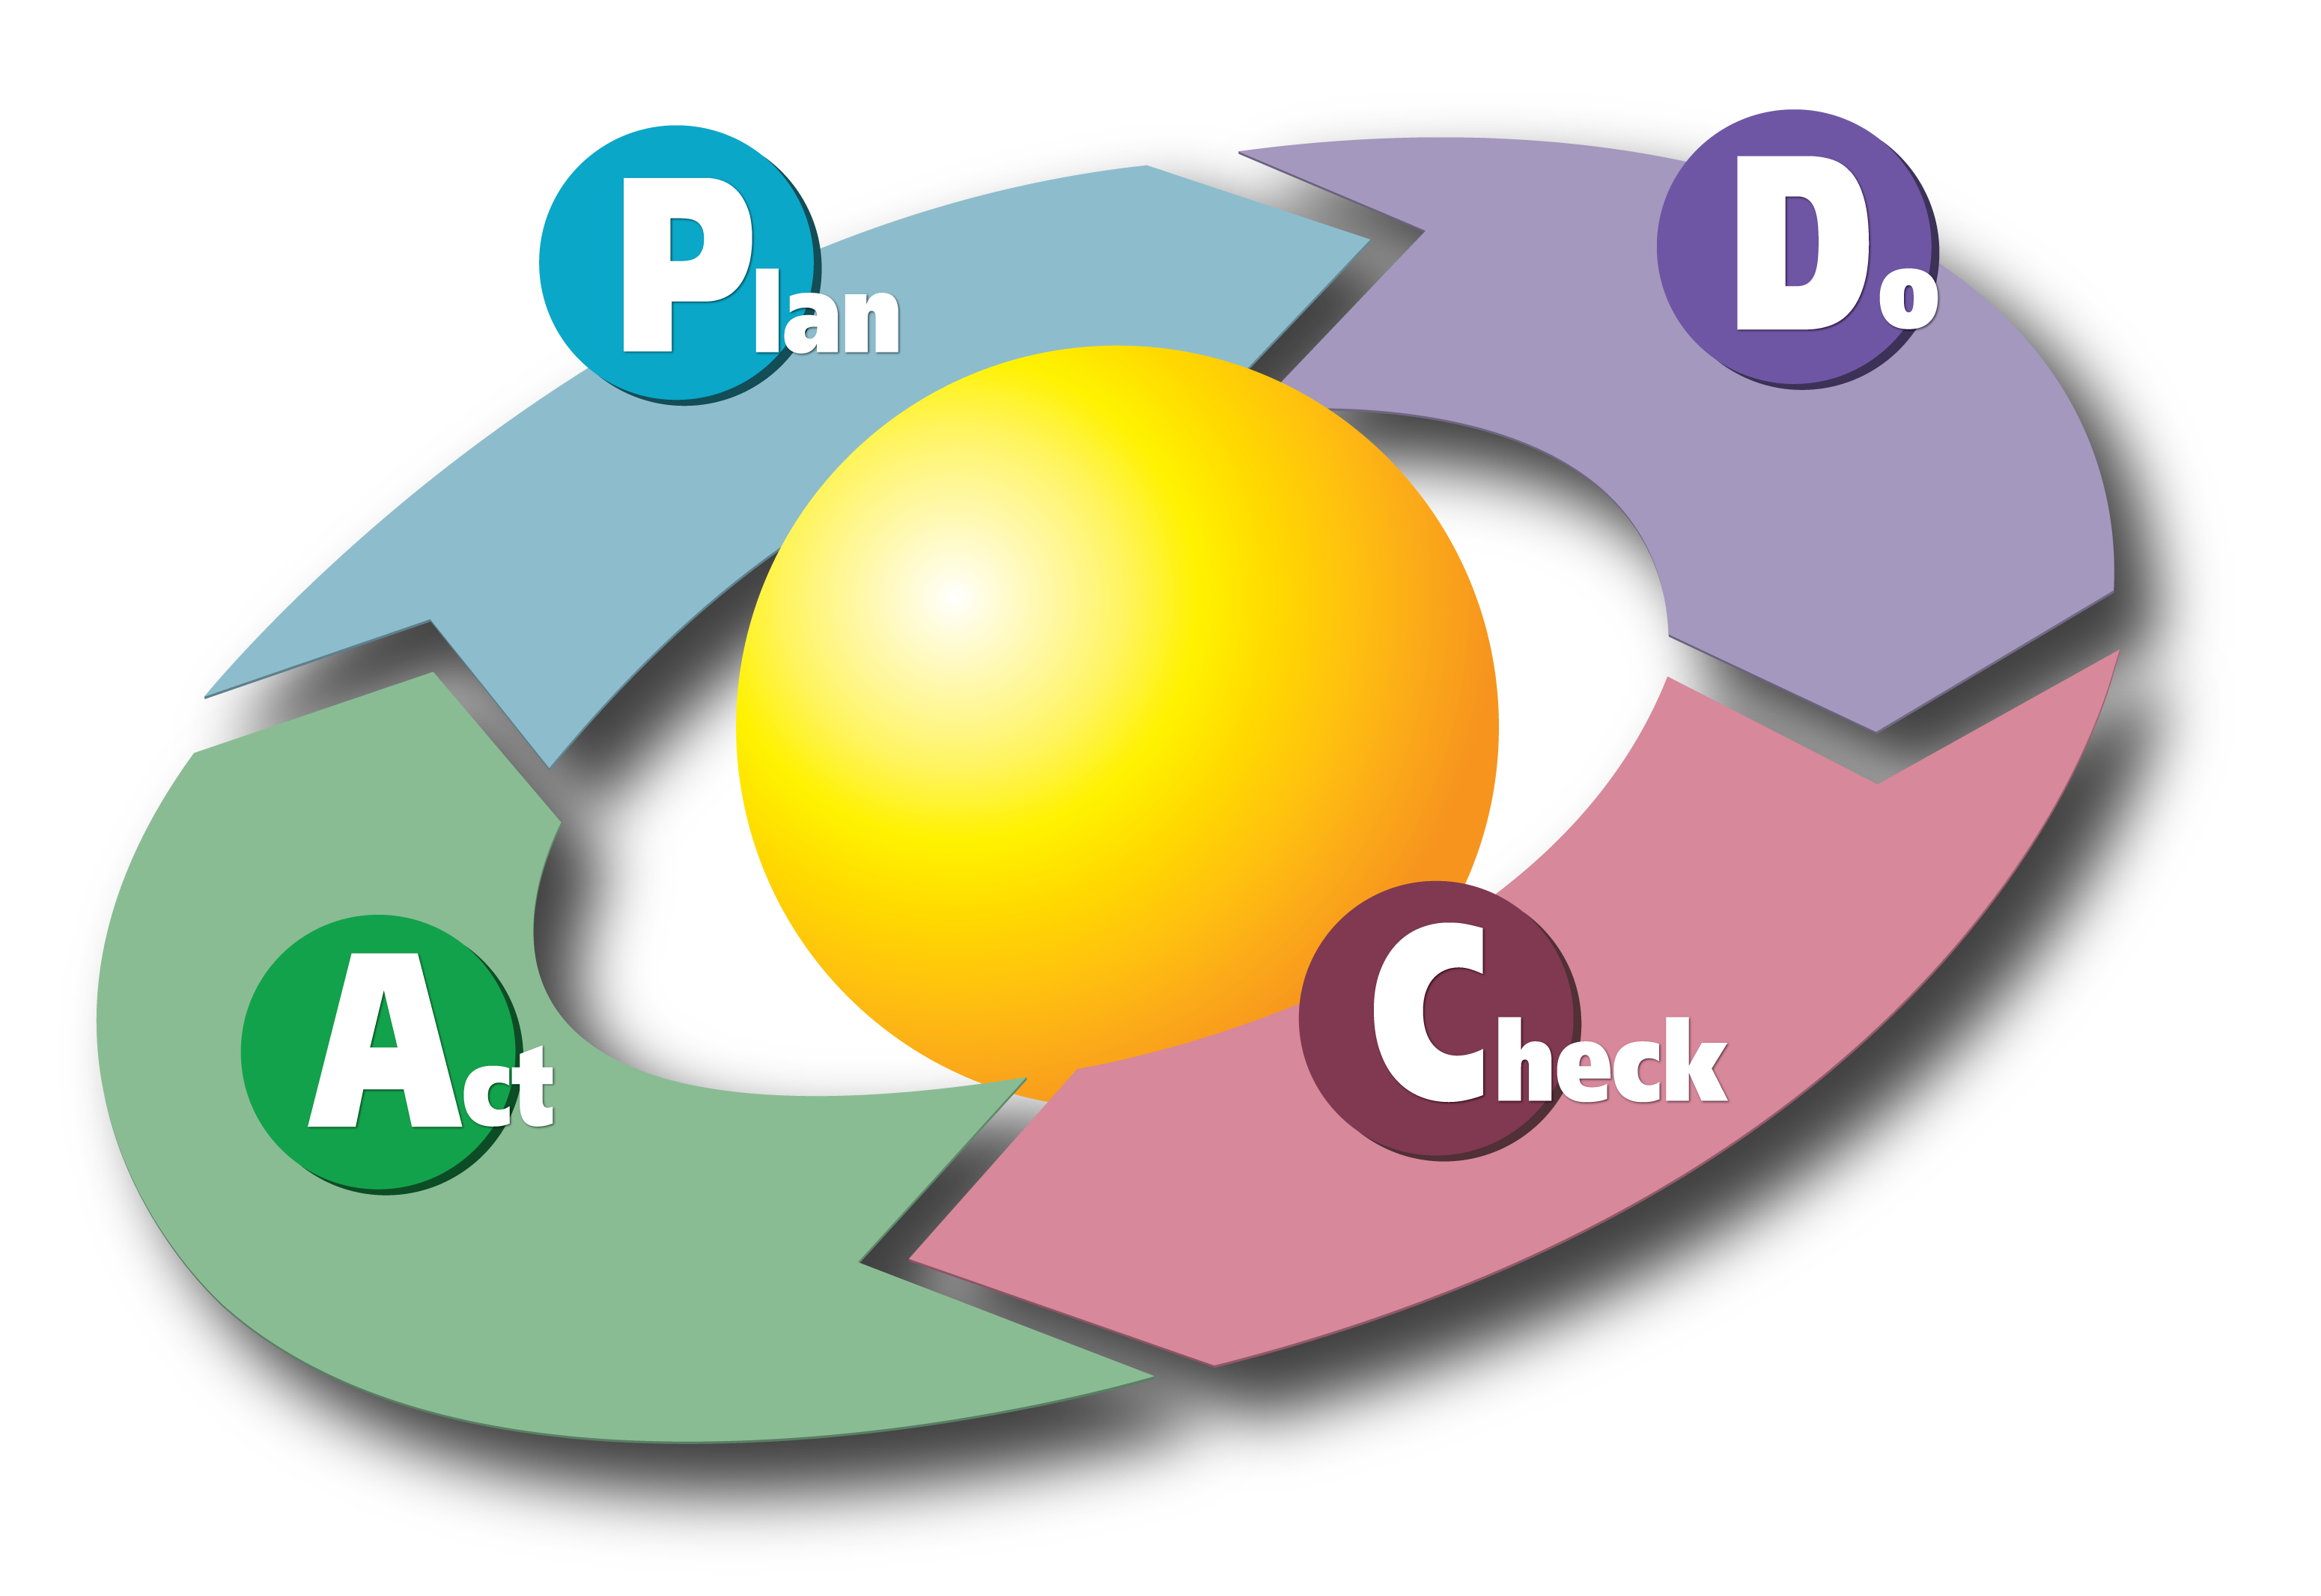
\includegraphics[width=.35\textwidth]{pdca}
\caption{Il ciclo di Deming.}\label{fig:pdca}
\end{figure}

Tale tecnica è costituita dalle seguenti fasi:

\begin{tabularx}{.9\textwidth}{>{\bfseries\scshape}lX}
plan  & analizzare il problema e stabilire le attività, le tempistiche e i soggetti coinvolti;\\
do    & attuare dettagliatamente le attività pianificate;\\
check & verificare a consuntivo quanto preventivato nella pianificazione;\\
act   & nel caso in cui il controllo abbia rilevato discrepanze tra preventivo e consuntivo attuare misure correttive.\\
\end{tabularx}

È chiaro che gli obiettivi di qualità prefissati possono essere raggiunti tramite una adeguata pianificazione delle attività, che deve essere rispettata attentamente per poter permettere al team un'autovalutazione ed eventualmente l'adozione di misure correttive volte al miglioramento continuo e all'attuazione delle \underline{best practices}.  Solo in tal modo è infatti possibile ottenere un prodotto di qualità.
\clearpage

\section{Visione generale della strategia di verifica}

\subsection{Organizzazione, pianificazione strategica, pianificazione temporale e responsabilità}
Il processo di verifica inizierà quando il prodotto di un processo raggiungerà uno stadio che si potrà definire diverso da quello precedente. La verifica di tali cambiamenti sarà operata in modo mirato e circoscritta, grazie al registro delle modifiche che verrà compilato durante lo stilamento del documento stesso. Al termine della fase di verifica, i documenti saranno consegnati al responsabile di progetto, che provvederà ad approvarli.

Il team nel \underline{brainstorming} successivo all'analisi generale del progetto MyTalk ha deciso di adottare un ciclo di vita incrementale (specificato nel Piano di Progetto).

Coerentemente a tale scelta, il processo di verifica adottato opererà nelle diverse fasi del progetto nel modo seguente:

\begin{description}
	\item{\scshape\bfseries Analisi dei Requisiti:} Quando un documento uscirà dalla fase di redazione, verrà preso in esame ed effettuata una fase di revisione definitiva prima di essere presentato ufficialmente alla RR: 
\begin{itemize}
		\item Verrà presa in esame la correttezza grammaticale, che al contrario di quella ortografica può essere verificata solo mediante un accurata rilettura da parte del verificatore designato.
		\item Verrà presa in esame la correttezza lessicale mediante un'accurata rilettura da parte del verificatore designato.
		\item Verrà presa in esame la correttezza dei contenuti e la coerenza rispetto al documento mediante un accurata rilettura da parte del verificatore designato.
		\item Verrà effettuata la verifica che ogni tabella o figura sia corretta nel suo contenuto e disponga della rispettiva didascalia.
		\item Verrà presa in esame la correttezza rispetto alle Norme di Progetto redatte, utilizzando gli strumenti più appropriati per la verifica.
		\item Verrà presa in esame la corrispondenza tra ogni requisito e i Casi d'Uso, consultando e controllando le apposite tabelle di tracciamento, verificando inoltre la corretta gestione di entrambi mediante l'applicativo web creato appositamente da Software Synthesis.
		% corrispondenza tra i requisiti elencati e il capitolato
		% che i requisiti siano chiari, atomici, tracciabili (pag. 12 PdQ ZetaSolutions)
\end{itemize}
	\item{\scshape\bfseries Progettazione:} Il processo di verifica garantirà la rintracciabilità nei componenti individuati durante la fase di Progettazione di ogni singolo requisito descritto nell'Analisi dei Requisiti.
	% TODO:
	% aggiungere del nostro sistema di tracciamento fra requisiti e componenti
	% RELATIVAMENTE ALLA PROGETTAZIONE DI DETTAGLIO
	% test di unità (definizione, elementi richiesti, obiettivi: statement coverage e branch coverage)
	% test d integrazione
	\item{\scshape\bfseries Realizzazione:} I programmatori svolgeranno le attività di codifica del prodotto e i test di unità per la verifica del codice realizzato nel modo più automatizzato possibile. I verificatori inoltre controlleranno successivamente la presenza di eventuali errori o anomalie.
    % verifica funzionale (black-box) e verifica strutturale (white-box), citare Dijkstra relativente all'esito dei test
    % (possibilità di falso negativo)
	\item{\scshape\bfseries Validazione:} Alla fase di collaudo, il team garantirà il corretto funzionamento del prodotto MyTalk. Successivi \underline{difetti} riscontrati o eventuali caratteristiche non coerenti alle richieste dell'appaltatore saranno soggetti a modifica e correzione al fine di eliminare tali incongruenze. 
	% alpha test e beta test
\end{description}
\clearpage

\subsection{Risorse necessarie e disponibili}
L'utilizzo di risorse umane e tecnologiche è fondamentale per la verifica di qualità del prodotto e dei processi.

\subsubsection{Umane}
Software Synthesis si è imposta per garantire un elevato standard qualitativo che all'interno del team siano ricoperti, nel corso del progetto, i seguenti ruoli:

\begin{itemize}
\item Responsabile: responsabile della corretta realizzazione del prodotto secondo gli standard e le richieste commissionate, designato all'allocazione corretta delle risorse umane ai rispettivi compiti e stimolarne il coordinamento. 
Controlla inoltre la qualità dei processi interni mediante le attività di verifica da lui predisposte. Infine ha la facoltà di approvare o meno ogni proposta di correzione (migliorativa o di modifica generica) avanzata.
\item Amministratore: stila le metodologie e definisce le norme per la verifica dei processi, gestisce inoltre i risultati relativi ai test eseguiti e il processo di gestione e correzione delle anomalie e delle discrepanze.
\item Verificatore: applica i processi di verifica e validazione approvati dall'amministratore e predisposte dal responsabile tenendo traccia del suo lavoro. Ogni discrepanza o anomalia incontrerà durante tale attività verrà presentata tramite \underline{ticketing} (vedi capitolo 5).
\item Programmatore: durante il suo lavoro ha l'obbligo di risolvere le anomalie evidenziate tramite \underline{ticketing} dai verificatori o dai test effettuati sul codice da lui stesso prodotto.
\end{itemize}

\subsubsection{Software}
A livello software risulteranno necessari strumenti per permettere l'automatizzazione nell'analisi statica del codice prodotto, ai fini di ricavarne il maggior numero possibile di informazioni.

Risulteranno altrettanto utili ai fini dei test di unità legati al linguaggio di programmazione scelto dei \underline{Frameworks} specializzati, e degli strumenti per standardizzare (e automatizzare) i test sul prodotto finale nonché produrre dei resoconti appropriati sulle eventuali anomalie riscontrate.

Infine il team ha deciso di produrre un semplice programma basato su interfaccia Web per il tracciamento e la gestione dei requisiti in modo da rendere più standard e automatizzata possibile questa fase del progetto.

\subsubsection{Hardware}
Software Synthesis ha a disposizione oltre al materiale personale di ogni componente del team (Computer portatili e fissi) le strutture fisiche ed informatiche messe a disposizione dalla facoltà di informatica dell'Università degli Studi di Padova, quali laboratori didattici e le aule studio allocate negli stabili della Facoltà stessa.
\clearpage

\section{Strumenti, tecniche e metodi}

\subsection{Strumenti}\label{sec:tools}
Si riporta a continuazione un elenco dei principali strumenti per la verifica della qualità di cui intende avvalersi il team nell'arco dello sviluppo del progetto.\footnote{Si rimanda invece alle Norme di Progetto per un elenco degli strumenti utilizzati non strettamente in relazione con la verifica e il controllo qualitativo.}
\begin{itemize}
  \item \textbf{SynthesisRequirementManager}, il sistema di gestione dei requisiti realizzato da \team, avente lo scopo di rendere quanto più agevole gestire il tracciamento dei requisiti a tutti i livelli (requisiti-UC, requisiti-CI, ecc.) e, da un punto di vista prettamente qualitativo, assicurare la necessità e la sufficienza dei casi d'uso e delle componenti software (\url{www.softwaresynthesis.org});
 \item \textbf{lacheck} ($\geq 1.26$) per assicurare la correttezza sintattica e l'adozione delle \inglese{best practices} per i sorgenti \LaTeX{} nonché rilevare in modo semi-automatico le sviste non segnalate dal compilatore in quanto pur corrispondendo a codice ben formato nascondono errori tipografici sottostanti per es.~bilanciamento delle virgolette, spaziature scorrette per frasi terminate da un acronimo prima di un punto, mancato utilizzo di spazi insecabili, ecc. (\url{www.ctan.org/pkg/lacheck});
 \item \textbf{hunspell} ($\geq 1.3$) come correttore ortografico e analizzatore morfologico in fase di redazione della documentazione, scelto per la sua portabilità ma anche  perché alle sue librerie si appoggia l'applicativo \textbf{TexMaker} utilizzato per la stesura dei documenti \LaTeX{} (\url{http://hunspell.sourceforge.net});
 \item le utilità che costituiscono la suite di \underline{QA} del W3C al fine di verificare l'aderenza agli standard delle pagine web generate, in particolar modo gli strumenti online:
 \begin{itemize}
   \item \textbf{Unicorn} in qualità di strumento di validazione unificato (\url{http://validator.w3.org/unicorn});
   \item \textbf{CSS Valitatom Service} come utilità di validazione per i fogli di stile a cascata (\url{http://jigsaw.w3.org/css-validator});
 \end{itemize}
 \item gli strumenti per sviluppatori integrati in \textbf{Google \underline{Chrome}} (\url{https://developers.google.com/chrome-developer-tools}) e, in particolare:
   \begin{itemize}
   \item la sezione \underline{Sources} che rappresenta un'interfaccia al \underline{debugger} per il motore \underline{JavaScript} V8 e consente di impostare \underline{breakpoint} (assoluti o condizionali) per seguire l'esecuzione del codice passo passo (con le consuete funzioni di \underline{''step over''}, \underline{''step into''} e \underline{''step out''}) nonché arrestare temporaneamente l'esecuzione al sollevamento di un'eccezione (o di un'eccezione non controllata);
   \item la sezione \underline{Timeline} che permette di quantificare i tempi necessari al caricamento e all'esecuzione degli script, nonché di tracciare l'utilizzo della memoria e forzare l'invocazione del \inglese{garbage collector};
   \item  gli strumenti di benchmark accessibili dalla sezione \underline{Profiles}, vale a dire il profiler della CPU, che permette di ricostruire l'albero delle chiamate di funzione e la percentuale di utilizzo della CPU per ciascuna funzione, e il profiler dello heap, mediante il quale è possibile ispezionare il contenuto dello heap e salvarne delle rappresentazioni istantanee;
   \end{itemize}
  \item \textbf{FirebugLite}, un'estensione per \underline{Chrome} che consente di ispezionare gli elementi \underline{HTML} e la struttura del \underline{DOM} nonché di modificare in tempo reale i valori delle proprietà dei \underline{CSS} (\url{https://getfirebug.com/firebuglite});
  \item \textbf{SpeedTracer} uno strumento che consente di identificare i problemi di prestazioni nelle applicazioni web visualizzando una serie di metriche in tempo reale grazie all'analisi dei dati resi disponibili a livello di motore di rendering del \underline{browser} (\url{https://developers.google.com/web-toolkit/speedtracer});
  \item \textbf{JSLint} analizzatore statico di codice \underline{JavaScript} volto a rilevare e impedire l'adozione inconsapevole di ''\underline{worst practices}'' in fase di codifica (\url{http://www.jslint.com});
  \item \textbf{ApacheBench} per testare l'efficienza prestazionale dell'applicazione lato \underline{server} mediante la simulazione di un numero arbitrario di richieste da parte dei \underline{client} (\url{http://httpd.apache.org/docs/2.2/programs/ab.html});
  \item \textbf{Eclipse} \underline{IDE} multipiattaforma e cross-language, scelto in particolare come ambiente di sviluppo per la parte \underline{server} da realizzarsi in \underline{Java}, che include al suo interno funzionalità di debugging (\url{http://www.eclipse.org}) utili ai fini della \underline{QA};
  \item \underline{plugin} \textbf{Metrics} per Eclipse, estensione che permette di associare un valore su una scala di riferimento al soddisfacimento di una serie di parametri di qualità del codice sorgente o metriche, per cui si rimanda alla sezione \ref{sec:metrics} (\url{http://metrics.sourceforge.net});
  \item il \underline{plugin} \textbf{FindBugs} per Eclipse, al fine di effettuare analisi statica del codice a livello di bytecode alla ricerca di potenziali cause di \underline{malfunzionamento} (\inglese{bug patterns}) o adozione inconsapevole di `worst practices' (\url{http://findbugs.sourceforge.net});
  \item \textbf{JUnit} come framework per i test di unità da effettuarsi relativamente alla parte \underline{server} dell'applicazione (\url{http://www.junit.org});
\end{itemize}

\subsection{Tecniche}
Responsabili delle attività di controllo interne al gruppo sono i verificatori, che si presuppone essere in ogni caso e senza alcuna deroga distinti dai realizzatori del prodotto soggetto a verifica (programmatori o redattori di documentazione). Al fine di garantire la qualità, i verificatori sono tenuti all'utilizzo di due tecniche di analisi: statica e dinamica.

\subsubsection{Analisi statica}

L'analisi statica è un tipo di controllo basato sulla non esecuzione del codice, ma in senso lato può essere applicato a qualsiasi tipo di prodotto anche non propriamente eseguibile (ad es.~la documentazione di progetto). Sono previste, in particolare, due forme di analisi statica: il controllo manuale (detto altrimenti `desk check'') e il controllo assistito da strumenti automatici.

Per quanto concerne il \textbf{desk check}, cioè il controllo realizzato unicamente da parte di un agente umano, sono previsti due metodi formali:

\begin{itemize}
  \item \textbf{\underline{walkthrough}}: implica un esame ad ampio spettro del prodotto da verificare, che è preso in considerazione nella sua totalità in modo indiscriminato e senza alcuna assunzione previa sulla natura, la posizione e la frequenza degli errori da rilevare. Si tratta notoriamente di una tecnica molto onerosa in termini sia di tempo che di sforzo e può essere essa stessa per sua natura soggetta ad errori (in particolar modo falsi negativi). Tuttavia, almeno nelle fasi iniziali del lavoro, è l'unica scelta praticabile a causa della relativa inesperienza dei membri del gruppo nella realizzazione di prodotti complessi e articolati (sia software che documentazione). Allo scopo di ridurre il costo determinato dalla ripetizione di tale attività nell'arco di tutto il ciclo di vita è previsto che durante l'analisi in \underline{walkthrough} sia stilata una lista di controllo relativa agli errori più frequenti e ai contesti in cui è più probabile che si producano errori in modo da collezionare una base di esperienza comune e consolidata destinata ad alimentare le attività di ispezione.
  \item \textbf{\underline{inspection}}: prevede un controllo mirato avente obiettivi specifici, ristretti e stabiliti a priori \emph{prima} che la verifica abbia luogo. Si tratta di un'attività meno dispendiosa in termini di risorse perché non presuppone l'analisi esaustiva del prodotto ma è focalizzata su determinate categorie di errori frequenti, enunciate in una lista di controllo (\inglese{checklist}) redatta sulla base dell'esperienza personale e delle attività di \underline{walkthrough} precedentemente poste in essere.
\end{itemize}

La seconda forma di analisi statica prevede invece l'utilizzo di strumenti appositi denominati \textbf{analizzatori statici} e può essere svolta in modo semiautomatico senza richiedere necessariamente l'intervento di un umano. In particolare, come risulta dalla sezione \ref{sec:tools} si è stabilito di utilizzare degli analizzatori statici tanto per la parte documentale del progetto (come il comando \texttt{lacheck}) quanto per la parte propriamente eseguibile (JSLint per la parte \underline{JavaScript} e FindBugs per la parte \underline{Java}).

\subsubsection{Analisi dinamica}
I controlli dinamici, altrimenti definiti test, prevedono l'esecuzione del software in un ambiente controllato e con dati di input specificatamente pensati per testarne le funzionalità e l'aderenza ai requisiti mettendo in luce l'eventuale presenza di \underline{malfunzionamenti} dovuti alla presenza di \underline{difetti}. Caratteristica fondamentale dei test è la loro \emph{ripetibilità}, cioè dato lo stesso set di dati in ingresso e nello stesso contesto di esecuzione, l'output deve essere deterministico e univocamente determinato. Tale proprietà, unitamente all'auspicabile utilizzo di un \inglese{logger} che ha il compito di registrare le fasi dell'esecuzione del test, consente di individuare e riconoscere in maniera più agevole i \underline{difetti} presenti nel prodotto.

In base al loro ambito di applicazione, i test possono essere suddivisi in:

\begin{itemize}
  \item test di unità aventi come oggetto le singole unità e, oltre al modulo da verificare e ai dati d'esempio, possono coinvolgere anche componenti attive (\inglese{\underline{driver}}) o passive (\inglese{\underline{stub}}) che siano in grado di simulare le parti del sistema non ancora disponibili al momento in cui il test viene eseguito;
  \item test di integrazione atti a verificare la corretta interazione e integrazione fra le componenti che costituiscono le parti del sistema e hanno come risultato una \inglese{build}, vale a dire un sottosistema funzionante che può essere eseguito in modo indipendente;
  \item test di sistema, volti a testare il rispetto dei requisiti software individuati in fase di analisi dei requisiti da parte dell'intero sistema; 
  \item test di regressione destinati a rilevare il caso indesiderabile in cui una modifica locale destabilizza il resto del sistema, si tratta del numero minimo di test necessario per scongiurare tale eventualità senza per questo dover ripetere \emph{in toto} i test di unità e di integrazione;
  \item test di accettazione, o collaudo, realizzato sotto la supervisione del committente per verificare l'aderenza del prodotto ai requisiti utente di più alto livello.
\end{itemize}

\subsection{Misure e metriche}\label{sec:metrics}
Si riporta, senza pretesa di esaustività, un elenco delle principali metriche in riferimento alle quali il team di sviluppo si ripropone di valutare in modo univoco e quantificabile la qualità del prodotto relativamente alla parte di codifica:

\begin{itemize}
  \item numero di righe di codice esclusi commenti e annotazioni, considerato nella sua totalità (TLOC, \inglese{Total lines of code}) o piuttosto come corpo dei soli metodi (MLOC, \inglese{Method lines of code});
  \item numero di metodi (NOM, \inglese{Number of Methods}) e numero di campi dati di ciascuna classe (NOF, \inglese{Number of Fields});
  \item profondità di una classe nell'albero di derivazione (DIT, \inglese{Depth of Inheritance Tree});
  \item numero di metodi ridefiniti (NORM, \inglese{Number of OverRidden Methods})
  \item indice di specializzazione (IS), definito come \[
  IS := \frac{DIT \times NORM}{NOM}
  \]
  \item complessità ciclomatica (o complessità condizionale), un indice che misura all'interno di un metodo il numero di cammini distinti che il flusso di controllo può intraprendere nel codice sorgente incrementando un indice di 1 unità per ogni istruzione di branch (if, for, while, do case, catch, operatore condizionale ternario, operatori logici cortocircuitati);
  \item peso della classe (WMC, \inglese{Weighted Methods per Class}) definito come la somma della complessità ciclomatica di tutti i metodi membri di una classe;
  \item mancanza di coesione dei metodi di una classe (LCOM, \inglese{Lack of Cohesion of Methods}), un indice che misura quanto i metodi di una classe fanno riferimento ai campi dati della stessa, definito se $m(A)$ è il numero di metodi che riferiscono il campo dati $A$ come \[
  LCOM := \frac{\frac{1}{NOF}\left(\displaystyle\sum_{A\;\mathrm{attributo}}{m(A)}\right) - NOM}{1-NOM}
  \]
  \item indice di utilità (Ca, \inglese{Afferent Coupling}) definito come il numero di classi esterne al package che dipendono da una determinata classe;
  \item indice di dipendenza (Ce, \inglese{Efferent Coupling}), definito come il numero delle classi interne al package che dipendono da una classe;
  \item instabilità (I) definita come \[
  I := \frac{Ce}{Ca + Ce}
  \]
  \item astrattezza (a livello di progetto) dato dal rapporto fra il numero di classi astratte/interfacce e il numero totale di tipi;
  \item la metrica relativa a metodi e procedure $SFIN - SFOUT$, dove SFIN (\inglese{Structural fan-in}) è il numero di volte che tale metodo è invocato nel corpo di altri metodi e SFOUT è il numero di invocazioni di metodi esterni all'interno del metodo stesso (corrispondono a Ca e Ce rispettivamente);
  \item rapporto fra righe di commenti e righe di codice.
\end{itemize}

Altre metriche che saranno prese in considerazione sono la lunghezza dei metodi e il numero di parametri di ciascun metodo.

\subsection{Metodi}
Il processo di misurazione attraverso il quale è possibile valutare quantitativamente l'aderenza del prodotto agli standard di qualità è basato su un ciclo iterativo simile al \underline{PDCA}\@. In particolare, in una fase preliminare prevede che sia stabilita l'importanza e l'ambito di applicazione della misurazione, la selezione di metriche da adottare come si è fatto nelle precedenti sezioni e la pianificazione del momento nel ciclo di sviluppo in cui le misurazioni dovranno essere effettuate.

La parte operativa, cioè la quantificazione dei valori delle metriche di qualità, avviene lungo tutto l'arco del ciclo di sviluppo, con particolare attenzione alle fasi di progettazione di dettaglio e di test effettuati contestualmente alla codifica e in fase di accettazione/collaudo.

Al fine di evitare che la verifica della qualità sia un onere troppo gravoso in termini di risorse umane e di tempo, anch'esso deve essere sottoposto a misurazione in quanto attività di progetto (cioè la parte `check' del \underline{ciclo di Deming}): il tempo di lavorazione impiegato per attività di verifica e \underline{QA} dovrà dunque essere registrato in ogni momento, ed è prerogativa del responsabile di progetto adottare misure correttive qualora i tempi dovessero risultare eccessivi al punto da compromettere il rispetto delle scadenze stabilite nel piano di progetto.

In via preliminare, si prevede di utilizzare i seguenti metodi di analisi:
\begin{description}
\item{\textbf{analisi del flusso di controllo}} volta ad assicurare che il codice sia ben strutturato e non contenga punti non raggiungibili;
\item{\textbf{analisi del flusso dei dati}} per scongiurare l'utilizzo inconsapevole di variabili non inizializzate e rilevare variabili inutilizzate o `write-only';
\item{\textbf{analisi del flusso di informazione}} al fine di assicurare l'assenza di dipendenze fra valori di variabili incoerenti con quanto previsto in fase di design architetturale (a livello di modulo, di componente o di sistema nella sua totalità).
\end{description}

\clearpage
\section{Gestione amministrativa della revisione}

\subsection{Gestione anomalie e incongruenze}
Un anomalia è una deviazione dalle aspettative definite sul prodotto, per la loro gestione è stato pianificato l'utilizzo di un sistema di \underline{ticketing}.
Lo strumento scelto dal team è Codebase, (\url{http://www.codebasehq. com/}) che permetterà ad ogni verificatore di aprire un \underline{ticket} per ogni nuova anomalia riscontrata.
I \underline{ticket} sono strutturati nel modo seguente:
\begin{itemize}
\item \textbf{Titolo:} comprende il nome del file da modificare e una descrizione stringata dell'errore;
\item \textbf{Tipologia}: indica la tipologia del \underline{ticket} aperto, nel caso di anomalie di carattere tecnico sarà impostato a Bug.
\item \textbf{Categoria Errore:} individua macroscopicamente il tipo di errore preso in esame.
\item \textbf{Stato:} tiene traccia dell'attuale stato del \underline{ticket} ed è catalogato in cinque categorie:
\begin{itemize}
\item \textbf{Nuovo:} \underline{ticket} appena creato dal Verificatore, rappresenta lo stato iniziale di ogni nuova pratica.
\item \textbf{Accettato:} stato booleano che identifica l'approvazione da parte del Responsabile di Progetto e ne assegna la pratica ad uno specifico soggetto (vedi punto Responsabile Correzione).
\item \textbf{In gestione:} il soggetto assegnato si sta occupando del problema e della relativa correzione dell'anomalia riscontrata.
\item \textbf{Corretto:} l'anomalia è stata correttamente gestita e risolta, il Responsabile di Progetto può considerare il \underline{ticket} chiuso.
\item \textbf{Non Valido:} l'anomalia proposta dal verificatore viene respinta dal Responsabile di Progetto in quanto non sussiste o semplicemente è già trattata in un altro \underline{ticket}.
\end{itemize}
\item Priorità: determina la priorità con cui dev'essere gestita l'anomalia, può essere di tre tipi
\begin{description}
\item \textbf{Critica:} l'anomalia risulta essere ad un livello che non permette l'esecuzione del prodotto;
\item \textbf{Alta:} l'anomalia provoca diversi problemi nell'utilizzo del prodotto.
\item \textbf{Media:} l'anomalia si presenta di moderata priorità 
\item \textbf{Bassa:} l'anomalia permette la corretta esecuzione del programma, la sua gestione ha una bassa priorità generale.
\end{description}
\item Responsabile Correzione: selezionato dal Responsabile di Progetto, ha il compito di gestire e correggere l'anomalia.
\item Note: comprende informazioni dettagliate redatte dal soggetto che ha riscontrato l'anomalia. Può comprendere la descrizione dell'errata esecuzione del prodotto a causa dell'anomalia e il comportamento corretto atteso nonché il tempo stimato per la correzione del problema stesso. 
\item Tag: indicano i termini inerenti all'anomalia per rendere la ricerca e l'identificazione più rapida ed efficace possibile.
\end{itemize}

Quando il progetto MyTalk giungerà al termine del processo produttivo sarà stilato un documento che analizzerà tutti i test effettuati e i relativi risultati che una volta analizzato dal Responsabile di Progetto potrà certificare la correttezza del prodotto finale.

Trattiamo ora le \textbf{discrepanze}, ovvero degli errori di coerenza tra il prodotto che si è realizzato e quello atteso. Tale errore si presenta in una forma di diversa gravità in base a quanto la discrepanza si distanzia dal risultato atteso, tuttavia verrà trattata come una normale anomalia e gestita tramite \underline{ticketing}.

La discrepanza generalmente può essere identificata come un allontanamento dalle norme di progetto o dai requisiti specificati nella fase d'analisi, nel primo caso il Responsabile di Progetto notificherà all'Amministratore che prenderà le dovute contromisure; nel secondo si identificherà il requisito associato al problema e se ne valuterà la discrepanza e le relative modifiche correttive per renderlo coerente al requisito stesso.

\subsection{Procedure di controllo di qualità di processo}
La qualità del processo è basata su un ciclo continuo di miglioramento basato del processo stesso e sull'uso ottimale delle risorse disponibili. 
Per garantire questo miglioramento continuo, l'organizzazione dei processi si basa sul principio \underline{PDCA}. La verifica che i processi rispettino la pianificazione rispetto ai requisiti stilati e alle risorse disponibili avviene attraverso l'analisi costante delle misurazioni sul prodotto del processo stesso.
Se i risultati di tali verifiche evidenziano valori che denotano ad un peggioramento qualificativo da quelli prefissati nella pianificazione, si provvederà ad identificare e a stabilire le possibili soluzioni al problema che li ha generati, intervenendo in modo correttivo sul processo. \

Risulta evidente che è possibile intervenire in modo migliorativo su un processo a prescindere dalla rilevazione di problematiche su di esso. Tale miglioramento consiste generalmente nella riduzione di risorse temporali o fisiche utilizzate o ridurre i cicli iterativi garantendo l'esecuzione fedele del processo rispetto al piano, il mantenimento del suo grado di efficacia ma allo stesso tempo aumentandone l'efficienza.

\clearpage
\section{Resoconto delle attività di verifica}
In questa sezione verranno descritte, nel prossimo aggiornamento, in che modo sono state effettuate le attività di verifica e i loro relativi esiti.

\section{Prossima versione Piano di Qualifica}
E' stato preventivato che nella prossima versione del Piano di Qualifica (coerentemente alle norme di progetto redatte si tratterà della versione 2.0) saranno aggiornate le sezioni riguardanti:
\begin{itemize}
\item procedure di validazione del codice prodotto;
\item resoconto finale delle attività di verifica della fase di progettazione;
\item definizione definitiva degli strumenti software utilizzati.
\end{itemize}
\end{document}
